\chapter{Конструкторская часть}

\section{Алгоритм BFS}

Для проверки связности графа используется обход в ширину (BFS).
Схема последовательной и параллельной реализаций представлена на рисунках~\ref{fig:bfs-seq} и~\ref{fig:bfs-par}.

Оценка вычислительной сложности BFS:
\begin{equation}
T_{\mathrm{BFS}} = O\!\left(|V| + |E|\right),
\label{eq:bfs-complexity}
\end{equation}
где $|V|$ --- число вершин, $|E|$ --- число рёбер.

\begin{figure}[H]
    \centering
    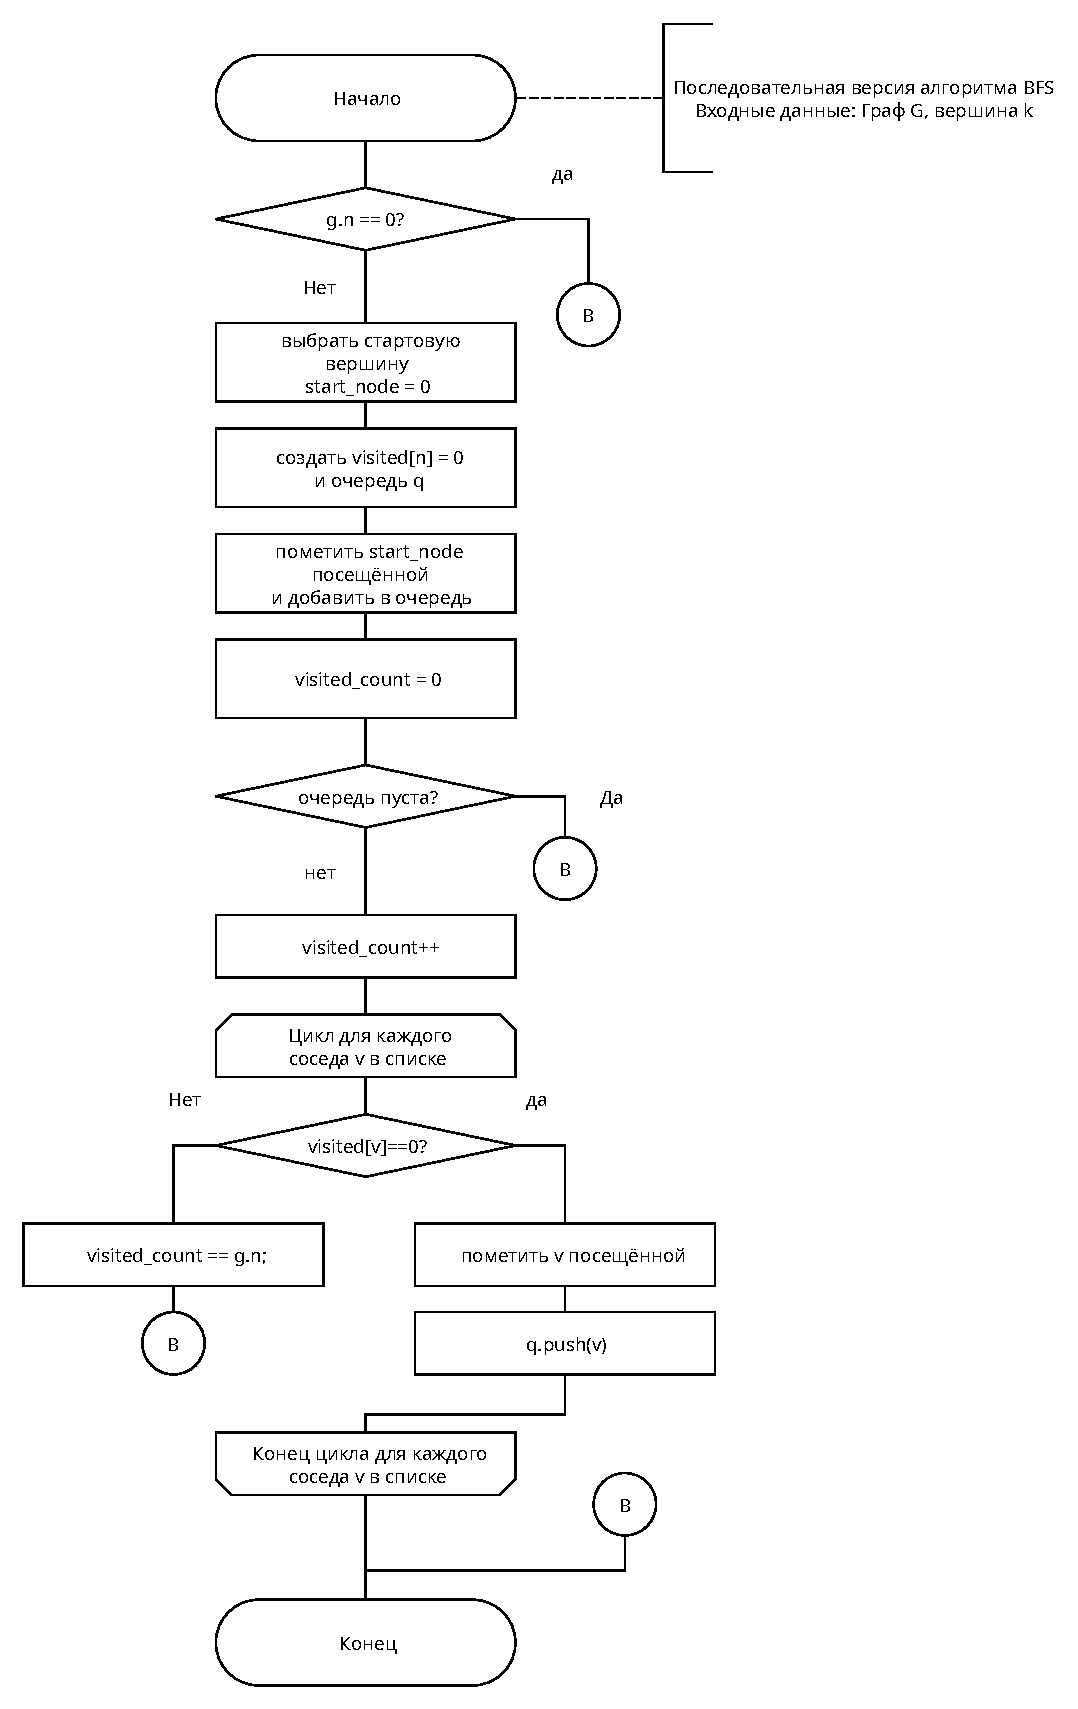
\includegraphics[width=0.78\textwidth]{images/schema_num1.pdf}
    \caption{Последовательная версия алгоритма BFS (проверка связности)}
    \label{fig:bfs-seq}
\end{figure}

\begin{figure}[H]
    \centering
    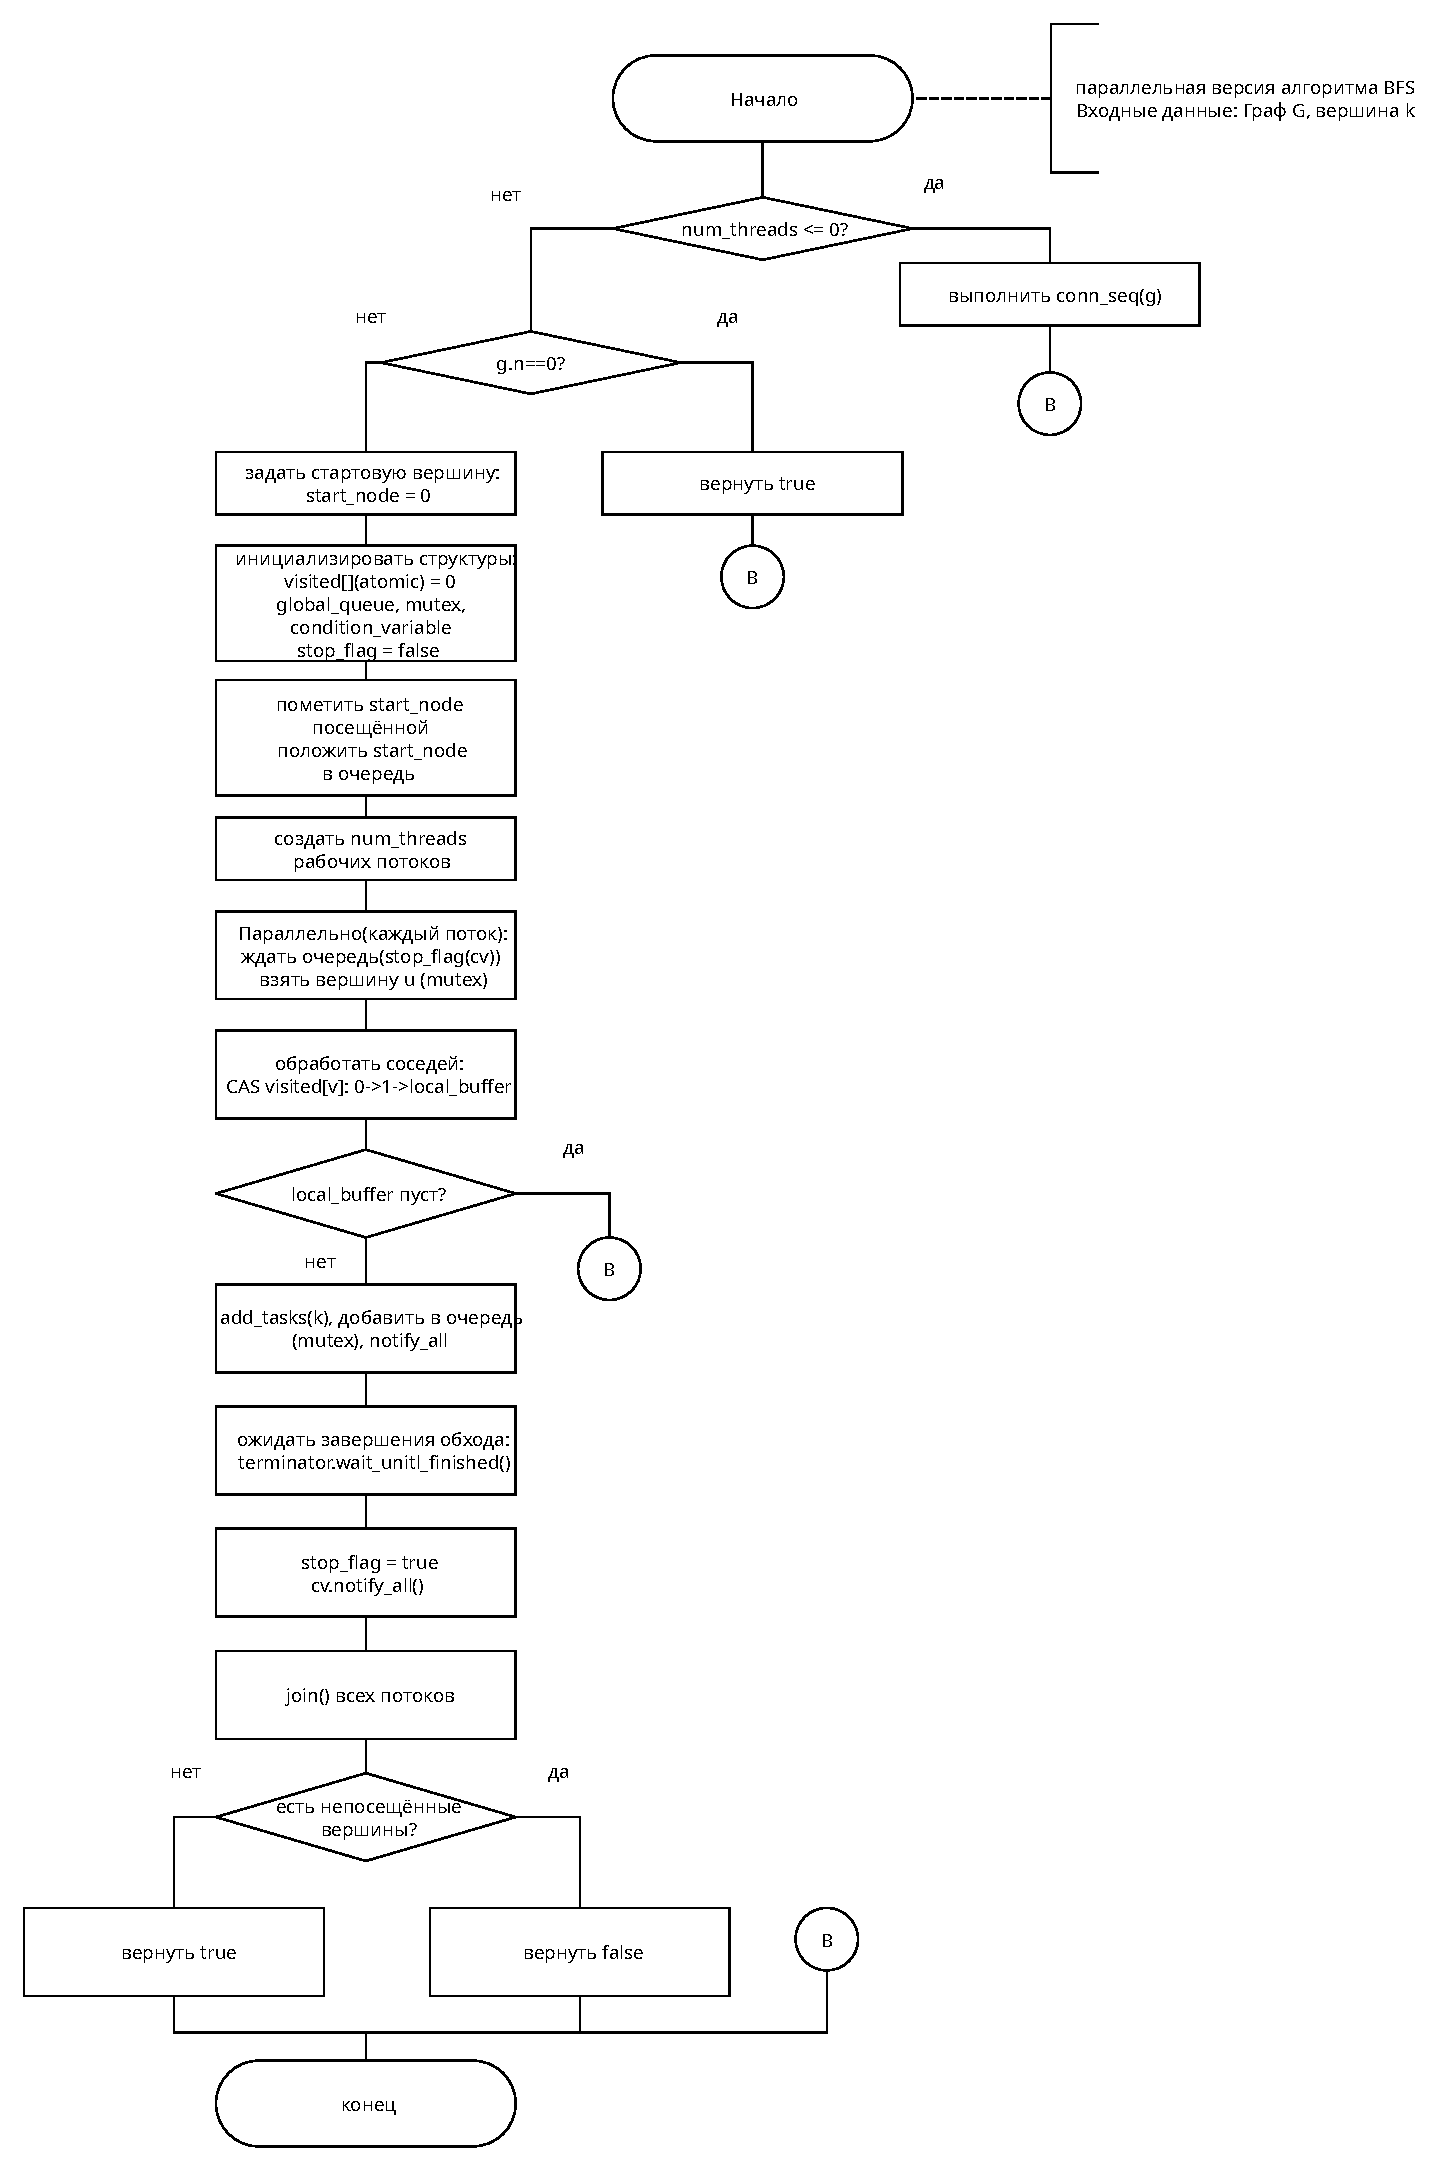
\includegraphics[width=0.78\textwidth]{images/schema_num2.pdf}
    \caption{Параллельная версия алгоритма BFS (проверка связности)}
    \label{fig:bfs-par}
\end{figure}


\section*{Вывод}

В данной части были разработаны последовательный и параллельный алгоритмы обхода графа в ширину (BFS), предназначенные для проверки связности графа.

\clearpage
